\chapter{Computational Methods} \label{chap:comp_met}

\section{Software: OpenFOAM and LIGGGHTS}
An implementation of the method provided in the Chapter \ref{chap:lit_rev} based on OpenFOAM\textsuperscript{\textregistered} \cite{jasak2007openfoam} open-source programming library which includes Finite Volume Method (FVM) solvers using its tools and data structures. A solver is made up of two main parts: a main structure and a number of extensions or tools. The main structure solves the governing equations, while the other part could be used for a specific tasks like: mesh decomposition, refinement or methods for solution of final system of equation. 
% i mean this will be methods for matrix inversion etc

Another part of the method is solving and coupling with OpenFoam solid movement part using Discrete Element Method (DEM) with LIGGGHTS\textsuperscript{\textregistered} package which is coupled with OpenFOAM through CFDEMcoupling \cite{kloss2011liggghts}. LIGGGHTS® is based on LAMMPS \cite{LAMMPS} a classical molecular dynamics simulator based on the time integration algorithm using Verlet symplectic integrator \cite{verlet}. The code is written in C++ and makes extensive use of templates. This design approach enhances the framework's flexibility and extensibility, enabling both users and developers to introduce custom algorithms, solvers, and utilities without modifying the core architecture. One other benefit of using LAMMPS, that it supports large scale parallelism. Distributed-memory parallelism via MPI with different ways of spatial decomposition. This all give opportunity to run the whole simulation in parallel on an HPC cluster.

\section{Parallel Computations}

For large problems, such as those found in industrial applications, calculations on a single processor would be too slow. Both OpenFOAM® and LIGGGHTS can be run in parallel using MPI, but some adjustments were needed for a parallel coupled computation. Originally, force calculations and particle locations were based only on information about the center of the body. This led to inaccurate results when the object crossed a processor boundary and should have been located on two processors at the same time.

In other words, for large problems, it is necessary to run OpenFOAM and LIGGGHTS in parallel on multiple processors. However, the challenge arises when particles move between interfaces of subdomains assigned to different processors, leading to potential errors. Such movement can induce velocity oscillations due to the inconsistent force calculations as particles move from one processor's domain to another. This issue must be carefully considered during the mesh decomposition phase to ensure that the domain is divided in a manner that minimizes these inaccuracies. In our experience, we encountered a challenge with velocity measurements in a straightforward scenario involving a falling sphere, where there was an unexpected spike in velocity. Upon investigation, it became clear that the issue stemmed from the sphere's position during mesh decomposition; it was situated precisely at the intersection of four domains. This unfortunate placement was the root cause of the velocity spike. Once we addressed this issue by adjusting the mesh to avoid such intersections, the results stabilized and showed strong agreement with previously published data, confirming the reliability of our simulations.

\section{Implementation:cfddemSolverMultisphereIB}
The schematic description is shown on the figure below \ref{fig:cfddemSolver}. 
\begin{figure}[!ht]
    \centering
    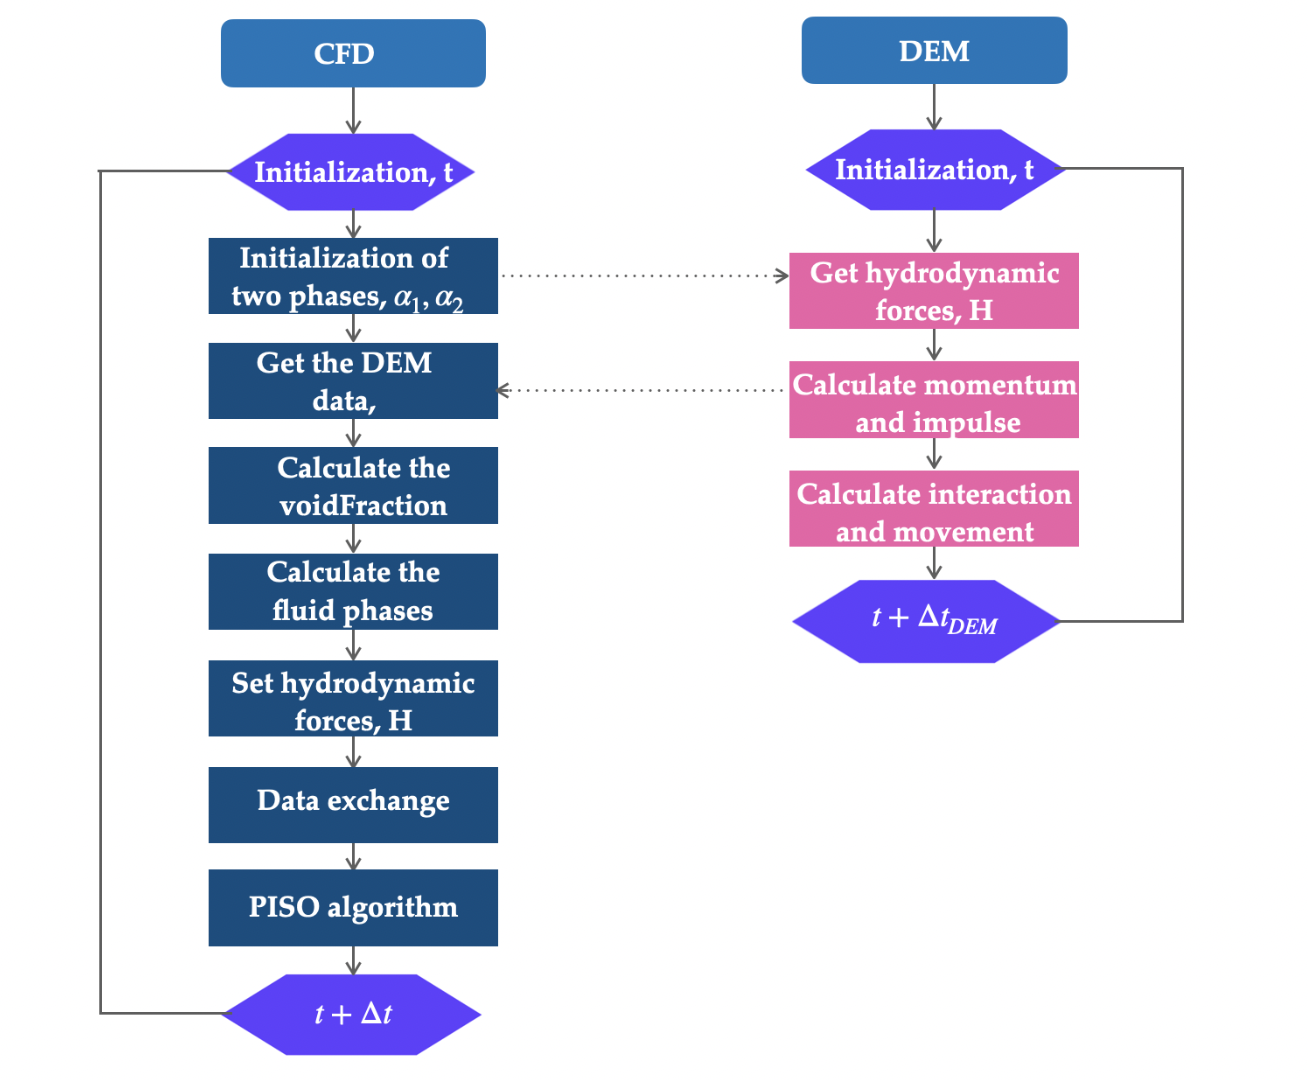
\includegraphics[width=16cm]{Images/chap4/CFD-DEM_scheme.png}
    \caption{Schematic description of CFD-DEM solver.}
    \label{fig:cfddemSolver}
\end{figure}

After initialization of DEM and CFD, we send DEM data to CFD part. Identify cells occupied with solid bodies and save this cells as a \textit{voidFraction} field. At the same time we initialize two phases, marking each cell of CFD in the range $[0,1]$ based on IsoAdvector method \cite{roenby2019isoadvector}

Then we starting PISO loop. First, solve momentum equation based on velocity fluid field from previous step with two phases and \textit{voidFraction} field also from the previous step or based on initial conditions, excluding pressure field.

The step of force calculation is the most important part of the simulation. Force calculated in function \verb|IBpressureForce::setForce()|. Where we should first initialize pressure, then for all cells which we found related to the DEM part on FVM mesh apply:
$$
F = - \nabla p \textbf{u}(1-voidFraction)
$$

\subsection{Time step calculation}
To run simulations with CFDEMcoupling we need to set up time step for DEM and for CFD solvers separately. It is common to use Courant (or Courant-Friedrichs-Lewy) number as a reference to get a solution converge. 

To calculate time step we will use relationship:
\begin{equation}
   \Delta t =  \frac{CFL \times \Delta x}{\mathbf{u}},
\end{equation}
where $\mathbf{u}$ - fluid velocity, $\Delta t$ - time step, $\Delta x$ - grid size and $CFL \in \mathbb{Q}$ is the Courant number. It indicates the number of cells a \textit{fluid particle} passes in one time step. Consequently, a calculation can only be considered stable if the Courant number is smaller or equal to one.

\subsection{Computational efficiency}
The algorithm presented on the Fig \ref{fig:cfddemSolver} is not straightforward. We need to pass back and forth data from one system to another. Thanks to API incorporated by a CFDDEM developers team, there was no need to develop this part. API works as as follows: 
\begin{itemize}
    \item set up equation which needed to be solved on fluid side
    \item create a force model with CFDDEM, calculate how solid body affect fluid.
    \item set up LIGGGHTS code, receive data form OpenFOAM through CFDDEM force model, calculate the solid body motion.
\end{itemize}

The software combination is takes a lot of resources and API is done using MPI. Moreover all process could be run parallel on CPU. When we are increasing the domain size, the number of CPUs required for running the simulation increased due to an increase in the finite volume mesh size.

The DEM calculations takes 1/8 of all computational time. The VOF part takes ~1/4 and parallel communication takes around same resources as DEM part. The main consumption, around half of all time, is coming from mapping the Lagrangian DEM data to a Eulerian field.  This step is critical for immersed boundary method, because velocity of the solid bodies is required to support continuous forcing approach.


\section{Validation and Verification}
We run of simulation to make sure that implemented solver work as we suppose. Otherwise we run validation experiment. For that reason we choose three different type of experiments:
\begin{itemize}
    \item \textbf{A falling sphere example, 1 phase}. Experiment for one phase and one solid body. 
    \item \textbf{A falling multi-spherical body}. This will show that multi-spherical body in the shape of sphere act the same way as a simple sphere.
    \item \textbf{A bouncing sphere example, water-air}. Experiment with two phases and one solid body. Density of the body smaller than one of the phase which make the body bounce and do not sink.
    \item \textbf{A falling multi-spherical body} into a water. This will be good example of that solver works.
\end{itemize}

\subsection{A falling sphere example, 1 phase}
Based on the initial validation of the created numerical model, we conducted a comparison between a one phase falling sphere simulation and the results presented in \cite{nan2023high}. The simulation utilized parameters for both the fluid and particle, which are provided in Table \ref{table1-chap4}. Figure \ref{fig:1ph_exp} displays the simulation from \cite{nan2023high}, while Figure \ref{fig:1ph_exp_me} showcases the results of the current solver. Based on a visual analysis, it is evident that the velocity of the fluid field around both particles is nearly identical. Additionally, Figure \ref{fig:trajectory_1ph} presents a comparison of trajectory in the $z$-direction and velocity of the falling particle.

% you might consider adding the following elements:

% Statistical Analysis: Mention any statistical measures you used to quantify the similarity between your results and the published ones. For example, you could talk about the error percentage or correlation coefficients.

% Reynolds Number Range: Explicitly state the range of Reynolds numbers you tested, as the published work did, to show that your solver is versatile.

% Drag Coefficient: If applicable, discuss how the drag coefficient in your simulation compares with the published results.

% Limitations: Briefly note any limitations or discrepancies between your model and the published work, and suggest possible reasons.

% Solver Strengths: Highlight any advantages your solver may have over the one in the published work, such as computational efficiency or the ability to handle more complex geometries.

% Future Work: Indicate what further validations or improvements could be made to your solver.

\begin{table}[ht]
    \centering
    \caption{Simulation Parameters} \label{table1-chap4}
    \begin{tabular}{llr}
        \toprule
        \hline
        Simulation Part         & Physical Parameters (units) & Value \\
        \hline
        \midrule
        Particle                 & Density (kg/m$^3$)          & 1200    \\
                         & Diameter (cm)          & 0.167    \\
                         & Initial height (cm)          & 3.5    \\
                         \hline
        Fluid                  & Density (kg/m$^3$)           & 1000   \\
                                & Viscosity (m$^2$/s)         & 1e$^{-6}$    \\
                                \hline
        \bottomrule
     \end{tabular}
\end{table}

\begin{figure}[!ht]
    \centering
    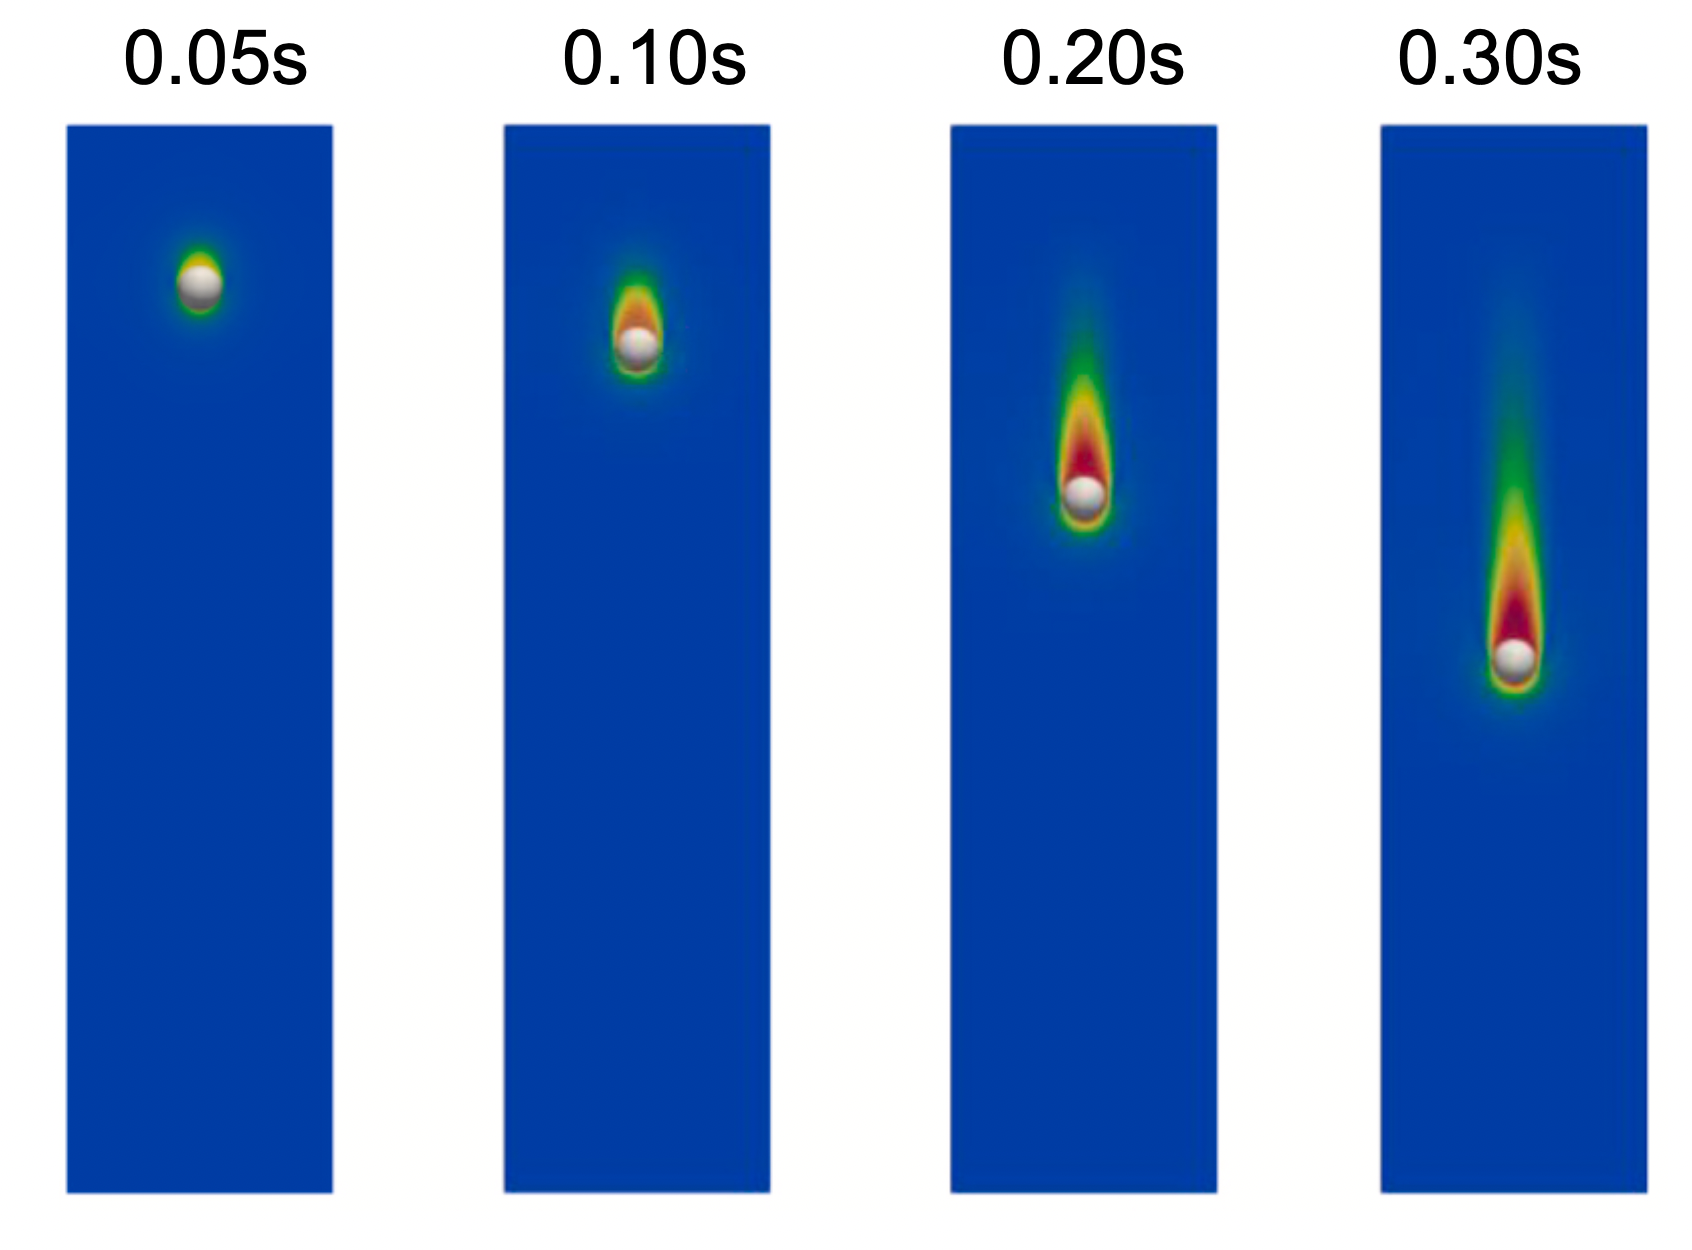
\includegraphics[width=10cm]{Images/chap4/1ph_exp.png}
    \caption{Falling sphere simulation in 1 phase fluid from the work \cite{nan2023high}.}
    \label{fig:1ph_exp}
\end{figure}

\begin{figure}[!ht]
    \centering
    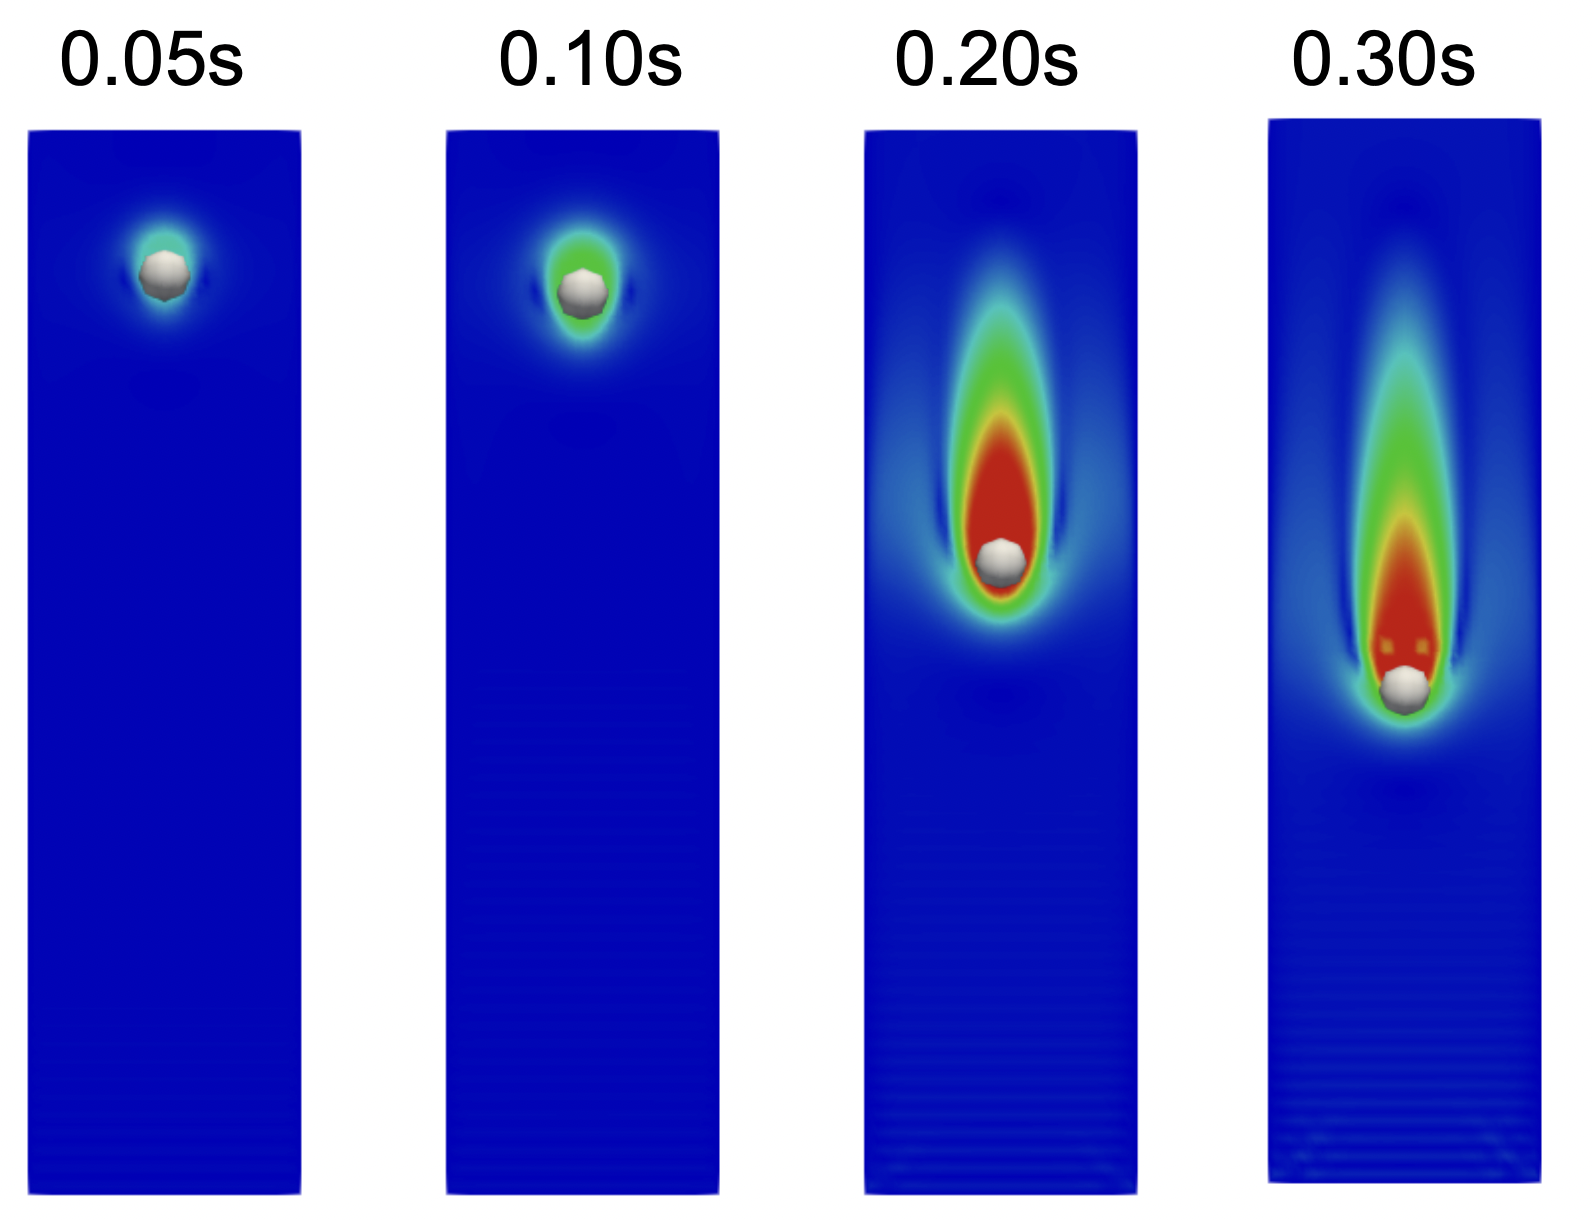
\includegraphics[width=10cm]{Images/chap4/1ph_exp_me.png}
    \caption{Falling sphere simulation in 1 phase fluid from the CFD-DEM simulation}
    \label{fig:1ph_exp_me}
\end{figure}

\begin{figure}[!ht]
    \centering
    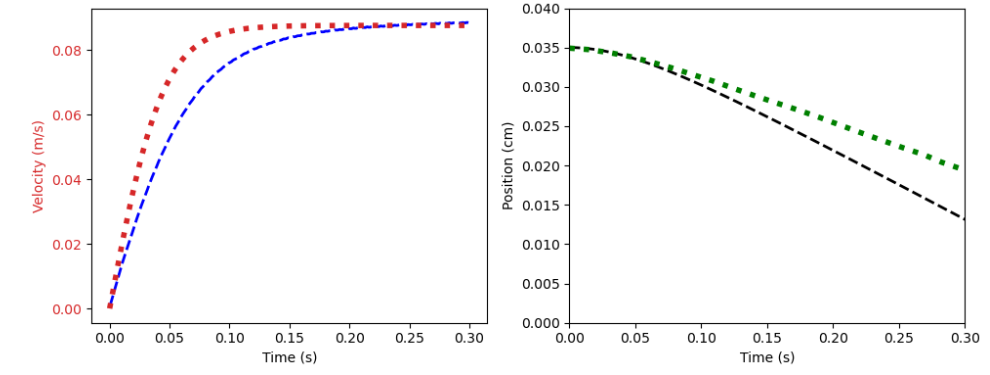
\includegraphics[width=16cm]{GWU_Thesis_Sarmakeeva/Images/chap4/falling_sphere_analytical.png}
    \caption{Falling sphere in 1 phase fluid 1) comparison in z-direction 2) velocity of the particle}
    \label{fig:trajectory_1ph}
\end{figure}
\newpage

\subsection{Multi-spherical falling sphere.}

In a subsequent validation phase, we extended the simulation to include a multi-spherical body designed to mimic the shape and dimensions of the single falling sphere. This experiment assessed the solver's capability to approximate complex particle shapes while maintaining the same fluid and particle parameters outlined in Table \ref{table1-chap4}.

Figures \ref{fig:multi_exp} and \ref{fig:multi_exp_me} present the simulation outcomes for the multi-spherical body from the published work and our solver, respectively. Qualitative analysis reveals that the fluid field velocity around the multi-spherical body closely mirrors the single sphere, reinforcing the solver's versatility in handling complex geometries.

For a more quantitative insight, Figure \ref{fig:trajectory_multi} displays the trajectory and velocity of the multi-spherical body in the $z$-direction. The data further corroborates the solver's accuracy and its applicability for simulating particles of varied shapes.

\section{The two phase validation} \label{ch-3}
\subsection{A bouncing sphere example, water-air}
The initial experiment comes from the work \cite{beck1987transient}. Where they using the tank parameters: length: 109.7 m, width 6.7 m, depth 3.2 m. The sphere radius $r= 0.254$ m , height $z = r/10$ above the free surface. The sphere density 500 kg/m .

First, we tried to make regular mesh similar to Pathak etc.\cite{pathak20163d} work. For the domain size from Pathak etc.\cite{pathak20163d} we followed formula:
\begin{equation}
    (length \cdot height \cdot width)  \cdot  r  \cdot  CPR,
\end{equation}
where CPR - cell per radius of sphere. To safe computational resources for tank %13\times 6.7 \times 3.4$ $\approx 17$ M cells with CPR $= 10$.
 $\approx 8$ M cells for tank $5\times 5 \times 5$, CPR $= 10$
 $\approx 2.7$ M cells for tank $5\times 5 \times 5$with mesh refinement to the center, CPR $= 10$

For the lowest mesh resolution results of simulation shown on the figure below \ref{fig:2ph_exp}.
\begin{figure}[!ht]
    \centering
    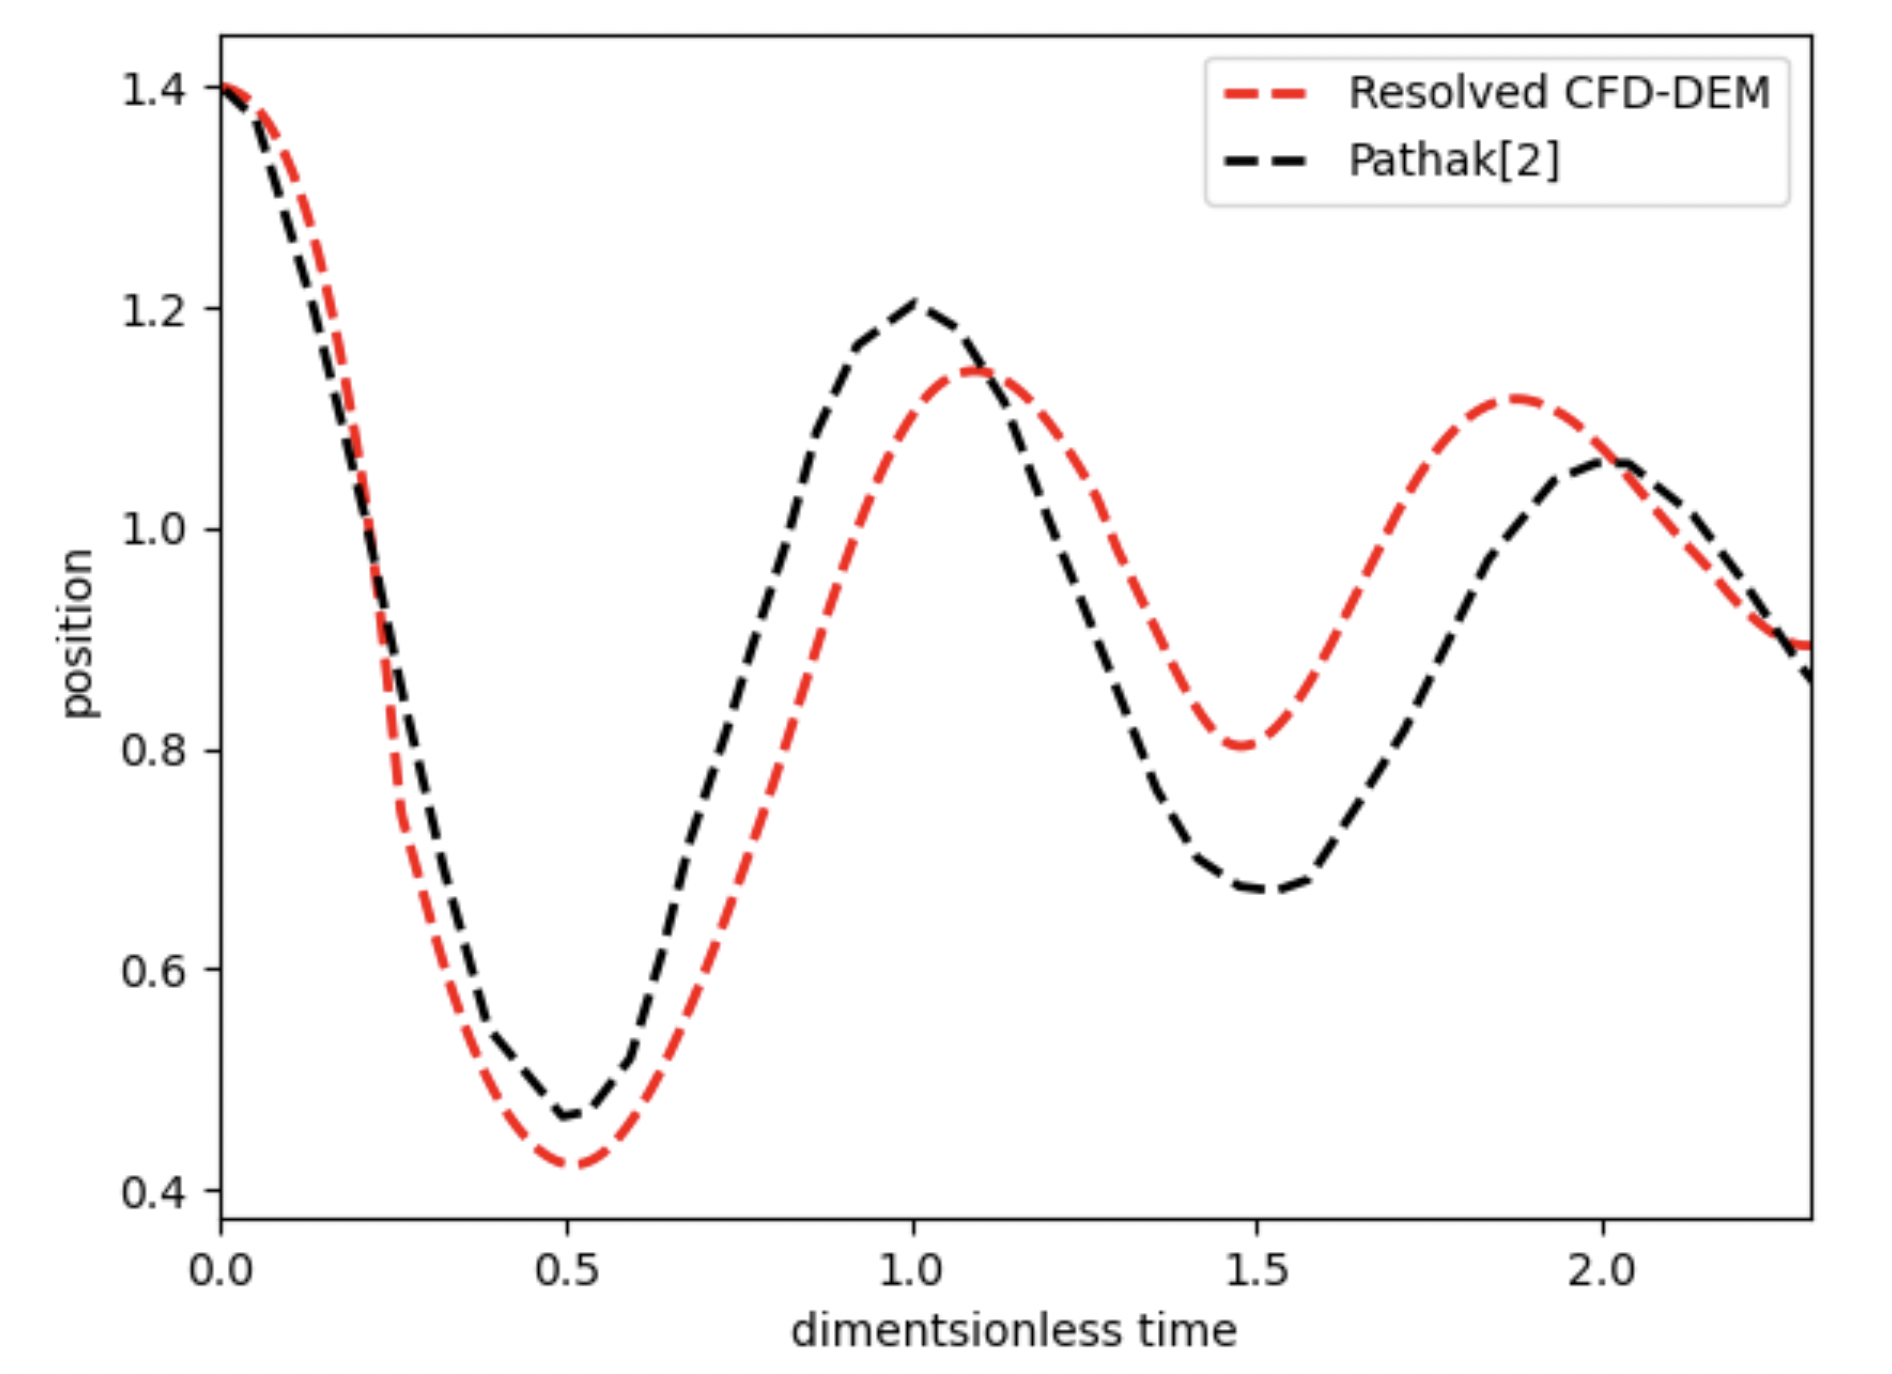
\includegraphics[width=10cm]{Images/chap4/bouncing_sphere_plot.png}
    \caption{Bouncing sphere simulation for two-phase fluid from the CFD-DEM simulation}
    \label{fig:2ph_exp}
    \end{figure}
The main parameters shown in the table below
\begin{table}[ht]
    \centering
    \caption{Simulation Parameters} \label{table2-chap4}
    \begin{tabular}{llr}
        \toprule
        \hline
        Simulation Part         & Physical Parameters (units) & Value \\
        \hline
        \midrule
        Particle                 & Density (kg/m$^3$)          & 500    \\
                         & Diameter (cm)          & $0.252$    \\
                         & Initial height (cm)          & $1.0252$    \\
                         \hline
        Fluid                  & Density (kg/m$^3$)           & $1000$   \\
                                & Viscosity (m$^2$/s)         & 1e$^{-6}$    \\
                                \hline
         Air                  & Density (kg/m$^3$)           & $1e-5$   \\
                                & Viscosity (m$^2$/s)         & 1e$^{-6}$    \\
                                \hline
        \bottomrule
     \end{tabular}
\end{table}


 \begin{figure}[!ht]
    \centering
    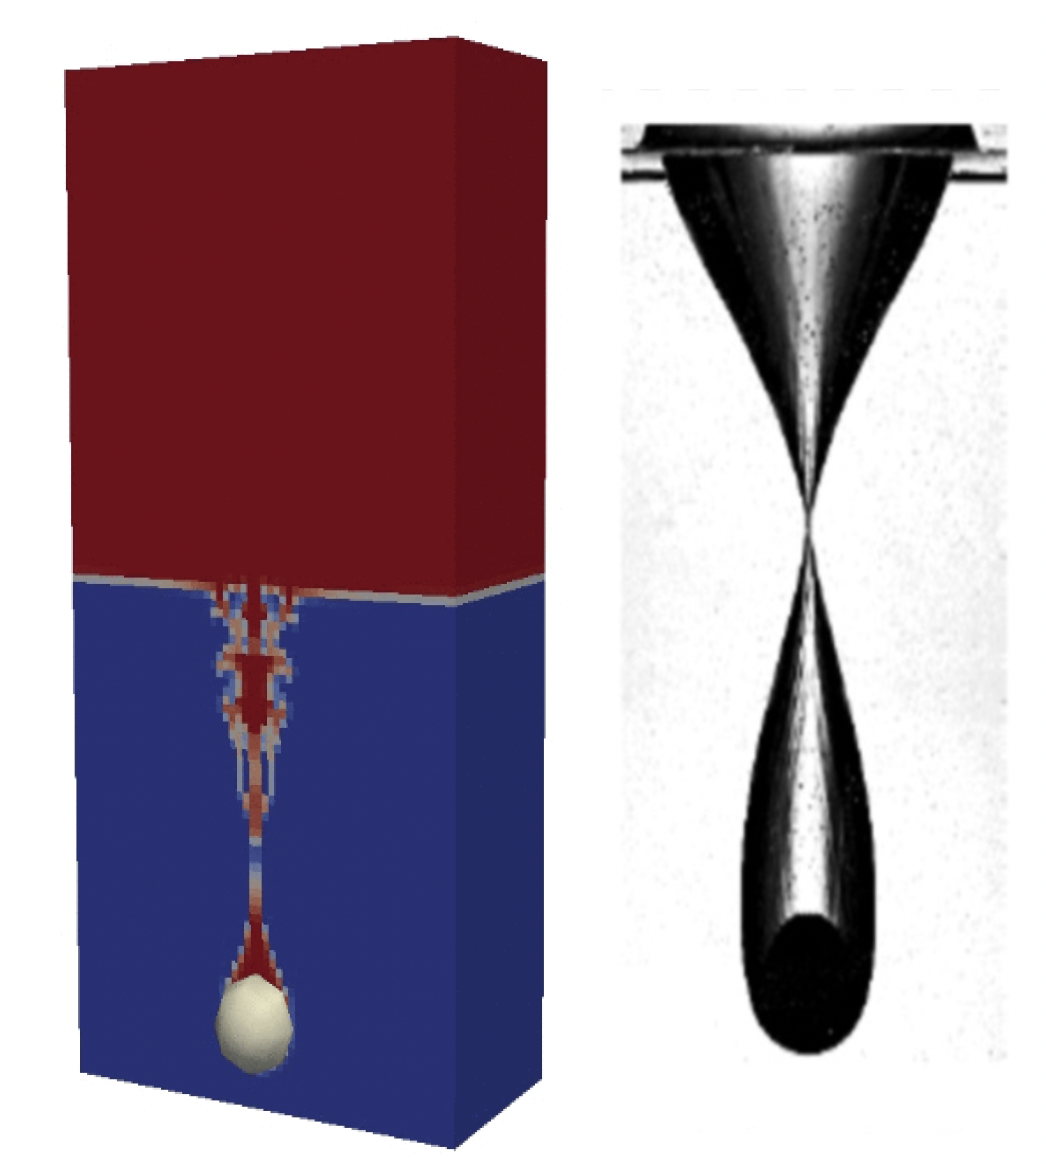
\includegraphics[width=12cm]{Images/chap4/cavityIB.png}
    \caption{Falling sphere visualization results. On the right, cavity after falling sphere in the water \cite{schwalbach}.}
    \label{fig:IB}
\end{figure}
Reproducing the physical experiments involving a sphere falling into the water, as outlined in \cite{schwalbach}, have challenges for numerical comparison. One primary obstacle is that the original paper needs to include the height from which the sphere is dropped. This parameter has a significant impact on the free surface during the simulation and is essential for ensuring the stability of our solver. Despite this, the trajectory of the falling sphere in our simulations aligns well with the physical experiments, suggesting that our results are both stable and comparable. Another study, \cite{shen2022resolved}, also attempts to replicate the original experiment through numerical methods. Again, this paper, in the same way, neglects to specify the height from which the spheres were dropped, making a complete comparison of results problematic.

Results of error with physical experiment compared with original experiment \cite{beck1987transient} and \cite{pathak20163d}.


\subsubsection{Computational setup}

For the numerical simulation we choose IsoAdvector \cite{roenby2019isoadvector} method for simulation of free surface which is described in a theoretical part. Applying second order Crank–Nicolson method for time differentiation . For interpolation  diffusion and convection terms we used scheme which called \textit{Gauss linear} in OpenFOAM, which is the second-order accurate scheme, the standard finite volume discretization using the Gaussian integration that requires the interpolation from cell centers to face centers. Pressure field tolerance was chosen as $1e-06$. With 3 PISO loops on each time step. The time step we choose $\Delta t = 1e-05$ for the VOF part and $\Delta t = 1e-06$ for the DEM part i.e communication was made every $10$ time steps from the solid body part.

\subsection{Multi-spherical body interaction with two-phase fluid}

The primary objective of this experiment is to illustrate initial stability and functionality of the developed CFD-DEM code through simulating the interaction of a multi-spherical body, analogous to a stone, with water.

The simulation involves a multi-spherical body consists out of 2 overlapping spheres, positioned at a $0.4$ m height above a fluid with the proprieties of water. The main properties are provided in the table below.
\begin{table}[ht]
    \centering
    \caption{Simulation Parameters} \label{table1-chap4}
    \begin{tabular}{llr}
        \toprule
        \hline
        Simulation Part         & Physical Parameters (units) & Value \\
        \hline
        \midrule
        Particle 1                & Density (kg/m$^3$)          & 500    \\
                         & Diameter (m)          & 0.25    \\
                         & Initial height (m)          & (0.5, 0.5, 1.4 )  \\
        Particle 2                & Density (kg/m$^3$)          & 500    \\
                         & Diameter (m)          & 0.25   \\
                         & Initial height (m)          &  (0.2, 0.4, 1.4)     \\
                         \hline
                                 Fluid                  & Density (kg/m$^3$)           & $1000$   \\
                                & Viscosity (m$^2$/s)         & 1e$^{-6}$    \\
                                \hline
         Air                  & Density (kg/m$^3$)           & $1e-5$   \\
                                & Viscosity (m$^2$/s)         & 1e$^{-6}$    \\
                                \hline
        \bottomrule
     \end{tabular}
\end{table}

The body is released and allowed to fall into the water under gravity forces. The simulation captures the motion of the body and the fluid's response upon impact and during the subsequent settling period. The results of simulation showed on a figure \ref{fig:two-phase exp} below.

\begin{figure}[!ht]
  \centering
  \begin{tabular}{cc}
    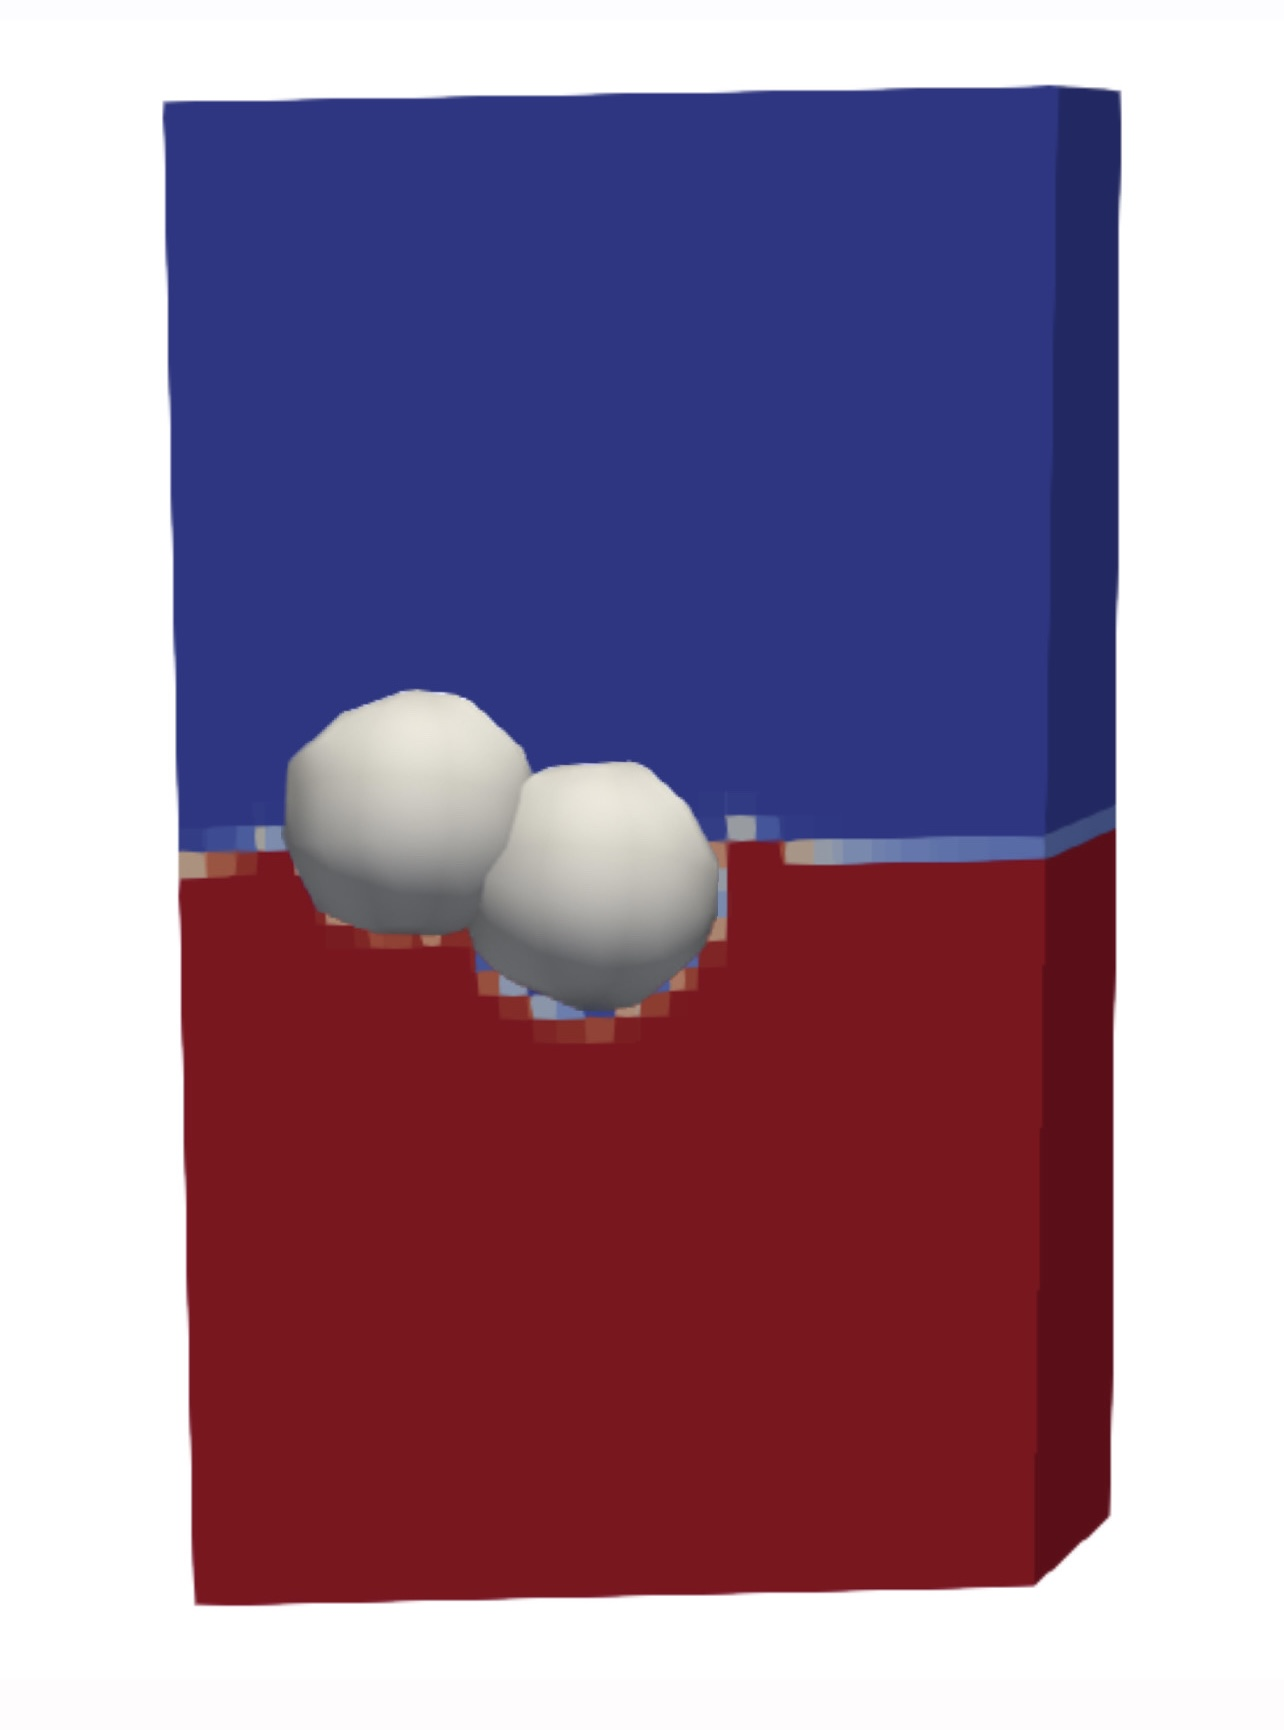
\includegraphics[width=0.4\textwidth]{Images/chap4/2_sph_2.jpg} & 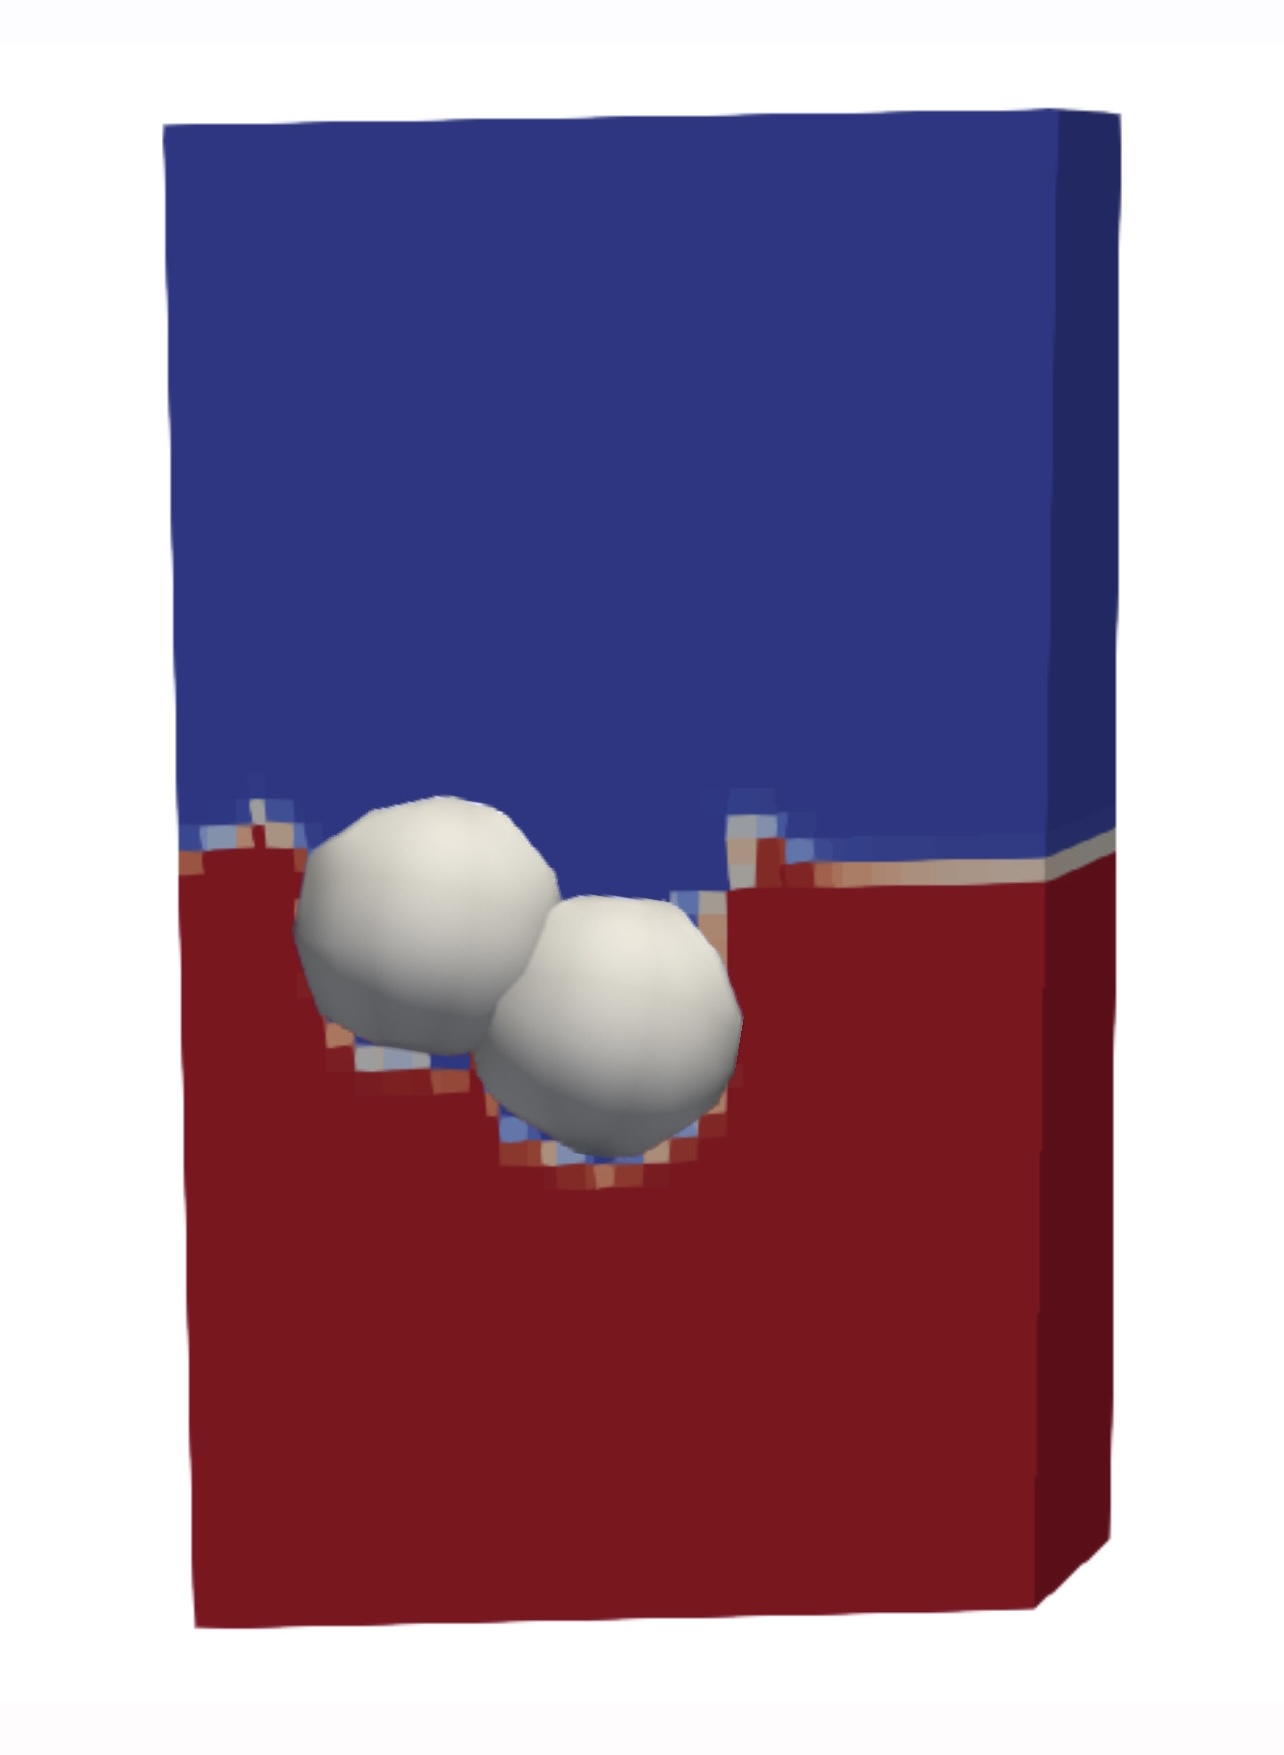
\includegraphics[width=0.4\textwidth]{Images/chap4/2_sph_1.jpg} \\
    %(a) 0. s & (b) 0.35 s \\
  \end{tabular}
  \caption{Falling 2 spheres.}
  \label{fig:two-phase exp}
\end{figure}
The results of simulation showed numerical stability of the solver. The main concern was the volume of fluid phases, it changes in the range less than 1\%. The future work and conclusion provided in the next section.

\subsection{Grid convergence analysis: Multi-spherical body interaction with two-phase fluid}

According to Roache's definition of code verification \cite{roache1998verification}, to confirm the ability to accurately solve the set of governing equations. A main strategy for validating the code is to convey a grid convergence study, which involves executing multiple simulations on successive finer grids. The discretization error is expected to approach zero asymptotically as the grid refined. The major point of interest in this context is the approximation order derived from the numerical method. For instance, if a second-order accurate method is used, it is reasonable to anticipate second-order convergence.

The discrepancy between the exact solution, denoted as $f_{exact}$, and the computed solution, represented as $f(h)$, as a result of the discretization error, can be expressed as follows:
\begin{equation}
f_{\text {exact }}-f(h)=c \cdot h^p+O\left(h^{p+1}\right)
\end{equation}


%\subsection{Methodology}%